\chapter{Overall experience}



\vspace{0cm}

My overall experience from this exercise has been very enlightening. I have become aware on a lot of issues which I didn't know about.

I got in touch with people from different people and had interesting conversations with them. 

I learned quite a few new things which I wouldn't have the chance to otherwise like:
\begin{enumerate}
\item When we try to solve any issue, we should not give a solution directly. We should consider all of its adversities before arriving at a decision otherwise our effort can have a negative effect.
\item To bring change, everyone has to change: adolescents, youth, adults, senior citizens. All the cogs of the clock have to function for it to show the right time. Even if one is malfunctioning, the entire balance is destroyed.
\item To help the society one must not necessarily have to go in the social service world but must try to bring some changes in himself.
\item We often dismiss social issues blaming the government, the system, the officials etc. but that in no way helps in solving them or giving a solution. We should try to put ourselves in the shoes of the person facing the difficulty and then consider trying to give a solution.
\end{enumerate}

I would definitely like to take part in another activity of this sort.

\newpage

\begin{figure}
	\centering
	\begin{subfigure}{.5\textwidth}
	  	\centering
	  	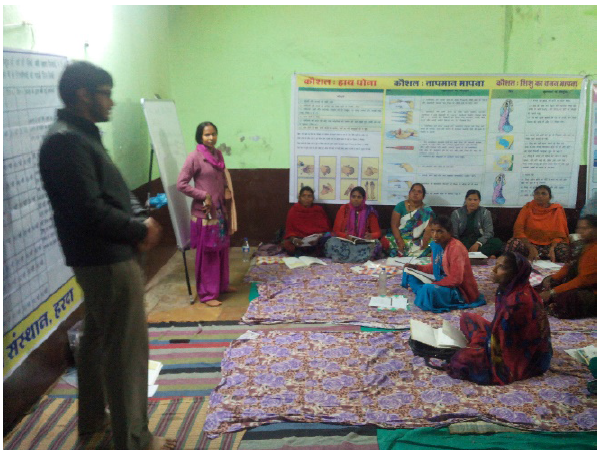
\includegraphics[width=2.45in]{Appendix1/im1.PNG}
	  	% \caption{Jalim Singh}
	  	% \label{fig:sub1}
	\end{subfigure}%
	\begin{subfigure}{.5\textwidth}
	  	\centering
	  	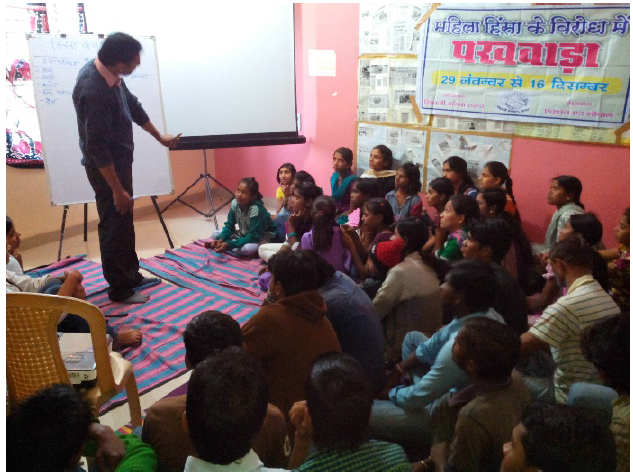
\includegraphics[width=2.45in]{Appendix1/im2.PNG}
	  	% \caption{Lokesh}
	  	% \label{fig:sub2}
	\end{subfigure}
	% \caption{Jalim and Lokesh - Case Studies}
	\label{figstart}
\end{figure}
\begin{figure}
	\centering
	\begin{subfigure}{.5\textwidth}
	  	\centering
	  	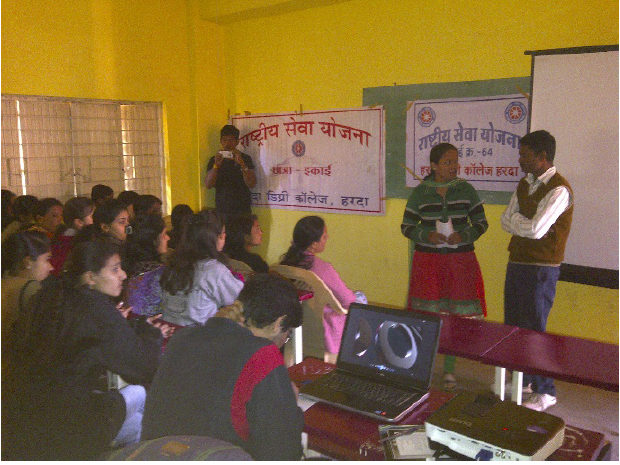
\includegraphics[width=2.45in]{Appendix1/im3.PNG}
	  	% \caption{Jalim Singh}
	  	% \label{fig:sub1}
	\end{subfigure}%
	\begin{subfigure}{.5\textwidth}
	  	\centering
	  	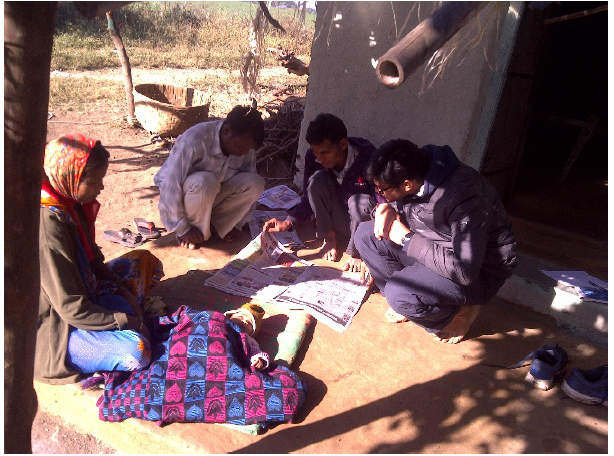
\includegraphics[width=2.45in]{Appendix1/im4.PNG}
	  	% \caption{Lokesh}
	  	% \label{fig:sub2}
	\end{subfigure}
	% \caption{Jalim and Lokesh - Case Studies}
	\label{figstart}
\end{figure}
\begin{figure}
	\centering
	\begin{subfigure}{.5\textwidth}
	  	\centering
	  	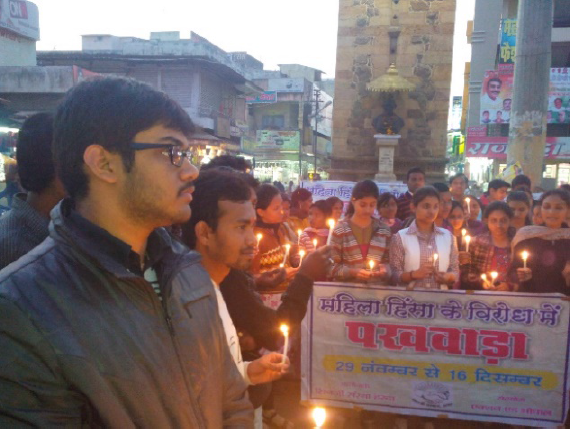
\includegraphics[width=2.45in]{Appendix1/im5.PNG}
	  	% \caption{Jalim Singh}
	  	% \label{fig:sub1}
	\end{subfigure}%
	\begin{subfigure}{.5\textwidth}
	  	\centering
	  	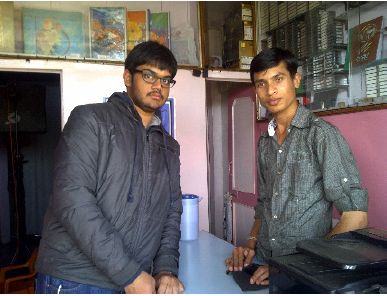
\includegraphics[width=2.45in]{Appendix1/im6.PNG}
	  	% \caption{Lokesh}
	  	% \label{fig:sub2}
	\end{subfigure}
	% \caption{Jalim and Lokesh - Case Studies}
	\label{figstart}
\end{figure}

\begin{figure}
	\centering
	\begin{subfigure}{.5\textwidth}
	  	\centering
	  	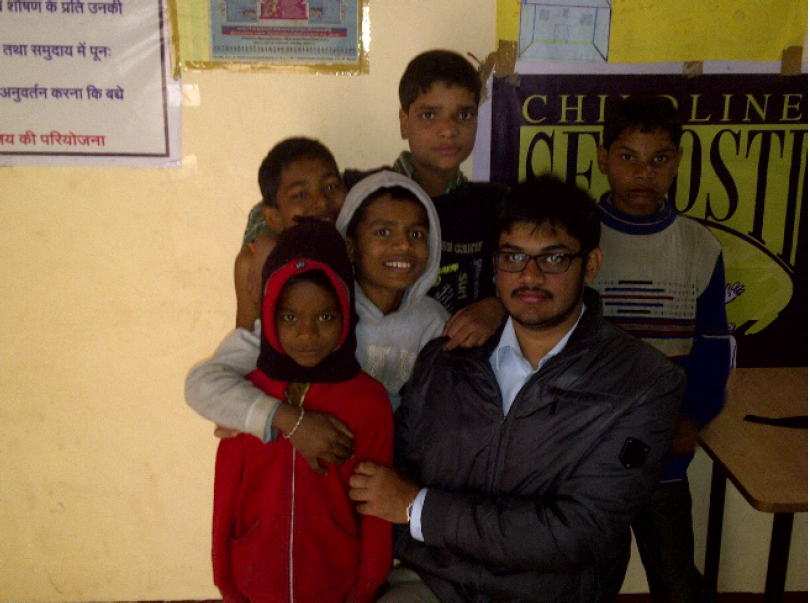
\includegraphics[width=2.45in]{Appendix1/im7.PNG}
	  	% \caption{Jalim Singh}
	  	% \label{fig:sub1}
	\end{subfigure}%
	\begin{subfigure}{.5\textwidth}
	  	\centering
	  	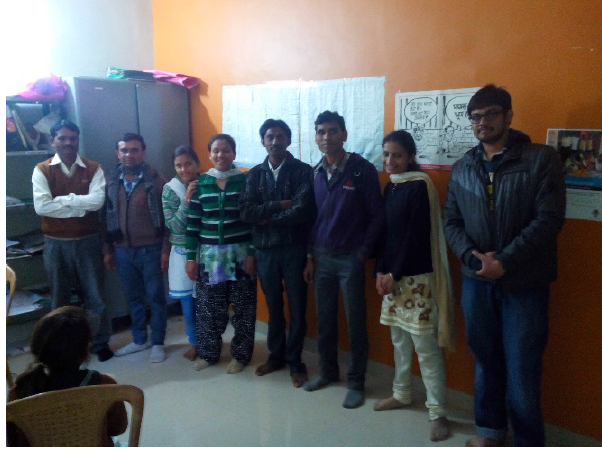
\includegraphics[width=2.45in]{Appendix1/im8.PNG}
	  	% \caption{Lokesh}
	  	% \label{fig:sub2}
	\end{subfigure}
	\caption{Some photos of the experience}
	\label{figstart}
\end{figure}


% ------------------------------------------------------------------------

%%% Local Variables: 
%%% mode: latex
%%% TeX-master: "../thesis"
%%% End: 
